\documentclass[12pt,twoside]{article}
\usepackage[noae]{Sweave}
\usepackage{caxetexFree}
\usepackage{lipsum}
\usepackage{titlesec}
\usepackage{bm}
\titleformat{\paragraph}[runin]{\normalfont\normalsize\textsb}{\theparagraph}{1em}{}
\newcommand{\myTitle}{Judicial behaviour part, 1}
\title{\myTitle}
\author{Chris Hanretty}
\date{6th May 2016}
\newcommand{\chaptermark}

%% From https://github.com/minrk/ipython/commit/325e76d80861d5cec65b08396c39c6316cde0912

    % commands and environments needed by pandoc snippets
    % extracted from the output of `pandoc -s`
    
    \DefineShortVerb[commandchars=\\\{\}]{\|}
    \DefineVerbatimEnvironment{Highlighting}{Verbatim}{commandchars=\\\{\}}
    % Add ',fontsize=\small' for more characters per line
    \newenvironment{Shaded}{}{}
    \newcommand{\KeywordTok}[1]{\textcolor[rgb]{0.00,0.44,0.13}{\textbf{{#1}}}}
    \newcommand{\DataTypeTok}[1]{\textcolor[rgb]{0.56,0.13,0.00}{{#1}}}
    \newcommand{\DecValTok}[1]{\textcolor[rgb]{0.25,0.63,0.44}{{#1}}}
    \newcommand{\BaseNTok}[1]{\textcolor[rgb]{0.25,0.63,0.44}{{#1}}}
    \newcommand{\FloatTok}[1]{\textcolor[rgb]{0.25,0.63,0.44}{{#1}}}
    \newcommand{\CharTok}[1]{\textcolor[rgb]{0.25,0.44,0.63}{{#1}}}
    \newcommand{\StringTok}[1]{\textcolor[rgb]{0.25,0.44,0.63}{{#1}}}
    \newcommand{\CommentTok}[1]{\textcolor[rgb]{0.38,0.63,0.69}{\textit{{#1}}}}
    \newcommand{\OtherTok}[1]{\textcolor[rgb]{0.00,0.44,0.13}{{#1}}}
    \newcommand{\AlertTok}[1]{\textcolor[rgb]{1.00,0.00,0.00}{\textbf{{#1}}}}
    \newcommand{\FunctionTok}[1]{\textcolor[rgb]{0.02,0.16,0.49}{{#1}}}
    \newcommand{\RegionMarkerTok}[1]{{#1}}
    \newcommand{\ErrorTok}[1]{\textcolor[rgb]{1.00,0.00,0.00}{\textbf{{#1}}}}
    \newcommand{\NormalTok}[1]{{#1}}
\providecommand{\tightlist}{%
  \setlength{\itemsep}{0pt}\setlength{\parskip}{0pt}}    
\pagestyle{fancy}
\renewcommand{\chaptermark}[1]{\markboth{#1}{}}
\fancyhead{} % clear all header fields
\fancyhead[CE]{\rightmark}
\fancyhead[CO]{\leftmark}
\fancyfoot{} % clear all footer fields
\fancyfootoffset[RO]{-0.25in}
\fancyfootoffset[LE]{-0.25in}
\fancyfootoffset[RE]{-0.25in}
\fancyfootoffset[LO]{-0.25in}
\fancyfoot[RO]{\thepage}
\fancyfoot[LE]{\thepage}
\fancyfoot[RE]{\texttt{\jobname{}.tex}, \textsf{revised \today}}
\fancyfoot[LO]{\texttt{\jobname{}.tex}, \textsf{revised \today}}

\renewcommand{\headrulewidth}{0pt}  %1.4

\setlength{\footskip}{33pt}

% Create headerless version for "plain" pages, 
% e.g., page 1 of a paper
\fancypagestyle{plain}{%
\fancyhf{} % clear all header and footer fields
\fancyfootoffset[RO]{-0.25in}
\fancyfootoffset[LE]{-0.25in}
\fancyfootoffset[RE]{-0.25in}
\fancyfootoffset[LO]{-0.25in}
\fancyfoot[RO]{\thepage}
\fancyfoot[LE]{\thepage}
\fancyfoot[RE]{\texttt{\jobname{}.tex}, \textsf{revised \today}}
\fancyfoot[LO]{\texttt{\jobname{}.tex}, \textsf{revised \today}}
\renewcommand{\headrulewidth}{0pt}
\renewcommand{\footrulewidth}{0pt}}

 \renewcommand{\leftmark}{\textsc{\caps{chris hanretty}}~~\(\cdot\)~~\emph{\textsb{%
\myTitle{}%
}}}
 \renewcommand{\rightmark}{\textsc{\caps{chris hanretty}}~~\(\cdot\)~~\emph{\textsb{%
\myTitle{}%
}}}



\begin{document}
\maketitle

\section{Introduction}\label{introduction}

\subsection{About this course}\label{about-this-course}

\begin{itemize}
\tightlist
\item
  to make inferences about judges from their behaviour
\item
  in two parts
\item
  regression-based methods
\item
  ideal point analysis
\item
  Regression based methods will start off with simple scenarios
\end{itemize}

\subsection{About me}\label{about-me}

\begin{itemize}
\tightlist
\item
  Reader in Politics, University of East Anglia
\item
  I've published on judicial politics in the UK and elsewhere
\item
  \emph{I am not a lawyer}
\end{itemize}

\subsection{About you}\label{about-you}

\begin{itemize}
\tightlist
\item
  I assume no knowledge of statistics
\item
  You may want to \emph{use} these models
\item
  I have provided \texttt{R} code for you
\item
  You may want to \emph{understand} these models
\item
  The code will still help
\end{itemize}

\subsection{Outline}\label{outline}

\begin{itemize}
\tightlist
\item
  Random assignment of a single judge to cases, with a continuous
  outcome
\item
  Random assignment of a single judge to cases, with a dichotomous
  outcome
\item
  Random assignment of multiple judges to cases, dichotomous outcome
\item
  Random assignment of multiple judges: some complications
\end{itemize}

\section{Continuous outcomes}\label{continuous-outcomes}

\subsection{Continuous outcomes in
law}\label{continuous-outcomes-in-law}

\begin{itemize}
\tightlist
\item
  Continuous outcomes are common

  \begin{itemize}
  \tightlist
  \item
    Fines (amount of fine in currency)
  \item
    Sentences (length of sentence in months)
  \item
    Damages (damages award)
  \item
    Negligence assessment (\% liability)
  \end{itemize}
\item
  Continuous outcomes are easy to model
\item
  We use the tools of linear regression
\end{itemize}

\subsection{Galton's children}\label{galtons-children}

\begin{figure}[htbp]
\centering
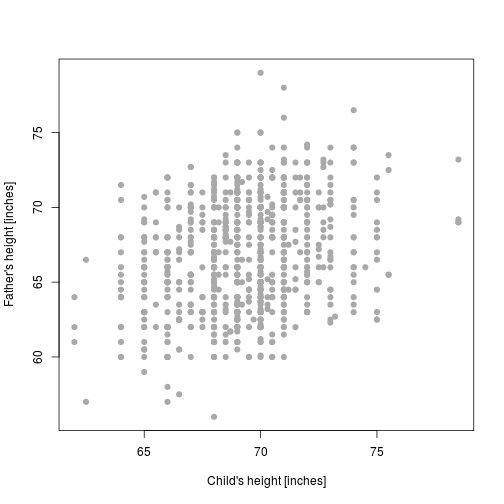
\includegraphics{figure/galtonfig-1.png}
\caption{Galton's height data}
\end{figure}

From: Galton, F. (1886). Regression towards mediocrity in hereditary
stature. \emph{The Journal of the Anthropological Institute of Great
Britain and Ireland}, 15, 246-263.

\subsection{A linear regression
equation}\label{a-linear-regression-equation}

\begin{itemize}
\tightlist
\item
  We can summarize the trend by using the equation for a straight line
\end{itemize}

\[
y = a + bx
\]

\begin{itemize}
\tightlist
\item
  I'll refer to

  \begin{itemize}
  \tightlist
  \item
    \(y\) as the dependent variable (in this case children's height)
  \item
    \(x\) as the independent variable (parents' height)
  \item
    \(a\) as an intercept
  \item
    \(b\) as a coefficient
  \end{itemize}
\end{itemize}

\subsection{The best-fitting line}\label{the-best-fitting-line}

\begin{figure}[htbp]
\centering
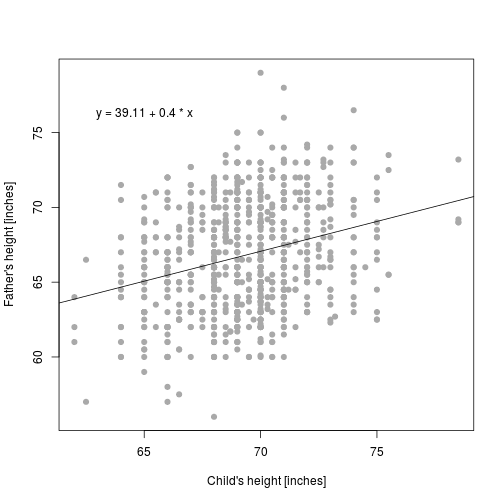
\includegraphics{figure/galton-bestfit-1.png}
\caption{Galton's height data}
\end{figure}

\subsection{Interpretation}\label{interpretation}

\begin{itemize}
\tightlist
\item
  When the value of the independent variable is zero, height is equal to
  \(a\) inches
\item
  For every unit increase in the independent, height increases by \(b\)
  inches
\item
  \ldots{} other things equal
\end{itemize}

\subsection{Interpretation}\label{interpretation-1}

\begin{itemize}
\tightlist
\item
  When the value of the independent variable is zero, height is equal to
  39.11 inches
\item
  For every unit increase in the independent, height increases by 0.4
  inches
\item
  \ldots{} other things equal
\end{itemize}

\subsection{For judges}\label{for-judges}

\begin{itemize}
\tightlist
\item
  Height can be measured by numbers
\item
  How can judges be measured by numbers?
\item
  Solution: create dummy variables
\end{itemize}

\subsection{An example}\label{an-example}

\begin{itemize}
\tightlist
\item
  Suppose cases are heard by two judges: Tender and Terrible
\item
  We set one of these judges as the \emph{reference category}
\item
  Suppose \emph{Tender} is the reference category
\item
  We create a dummy variable which has value zero if Tender heard the
  case
\item
  \ldots{} and one if \emph{Terrible} heard the case
\end{itemize}

\subsection{Graphing Tender and
Terrible}\label{graphing-tender-and-terrible}

\begin{figure}[htbp]
\centering
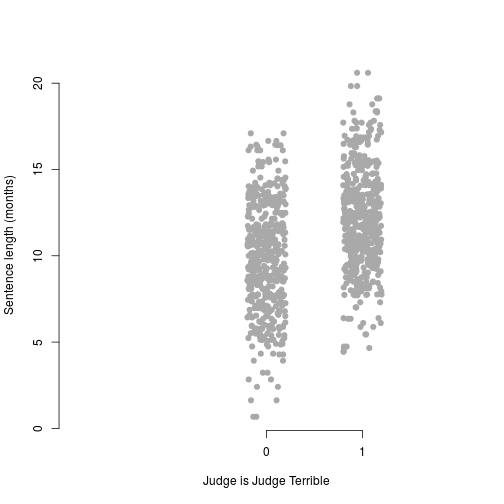
\includegraphics{figure/tendergraph-1.png}
\caption{Sentence lengths}
\end{figure}

\subsection{The best-fitting line}\label{the-best-fitting-line-1}

\begin{figure}[htbp]
\centering
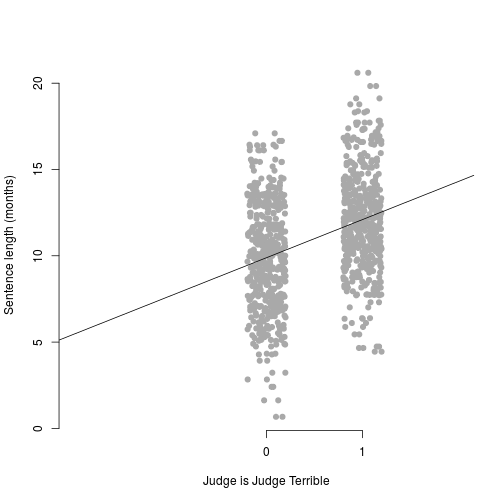
\includegraphics{figure/tenderbestfit-1.png}
\caption{Sentence lengths with best-fitting line}
\end{figure}

\subsection{Interpretation}\label{interpretation-2}

\begin{itemize}
\tightlist
\item
  When the value of the independent variable is zero (i.e., Tender heard
  the case), average sentence length is just under ten months
\item
  For each unit increase in the variable \texttt{terrible}, sentence
  length increases by 2.2 months
\item
  Alternatively: Judge Terrible imposes sentences that are 2.2 months
  longer than Tender.
\item
  This difference cannot be due to the cases heard by Terrible
\item
  if Terrible systematically heard cases which required longer
  sentences, no randomization!
\end{itemize}

\subsection{How does it look? The data}\label{how-does-it-look-the-data}

\begin{Shaded}
\begin{Highlighting}[]
\KeywordTok{head}\NormalTok{(tender)}
\end{Highlighting}
\end{Shaded}

\begin{verbatim}
##      Judge  Sentence JudgeTerrible
## 1 Terrible 16.595639             1
## 2   Tender 13.580389             0
## 3 Terrible 12.178373             1
## 4   Tender  4.746378             0
## 5 Terrible 15.378565             1
## 6   Tender 10.644786             0
\end{verbatim}

\subsection{How does it look? The
command}\label{how-does-it-look-the-command}

\begin{Shaded}
\begin{Highlighting}[]
\NormalTok{tender <-}\StringTok{ }\KeywordTok{read.csv}\NormalTok{(}\StringTok{"data/fakedata.csv"}\NormalTok{)}
\NormalTok{mod <-}\StringTok{ }\KeywordTok{lm}\NormalTok{(Sentence ~}\StringTok{ }\NormalTok{JudgeTerrible, }\DataTypeTok{data =} \NormalTok{tender)}
\end{Highlighting}
\end{Shaded}

\begin{itemize}
\tightlist
\item
  \texttt{mod}: an arbitrary name
\item
  \texttt{lm}: short for \emph{l}inear \emph{m}odel
\item
  \texttt{y\textasciitilde{}x}: dependent variable, then a tilde, then
  independent variables
\item
  \texttt{data=tender}: tell R where to find our data
\end{itemize}

\subsection{How does it look? The
output}\label{how-does-it-look-the-output}

\small

\begin{Shaded}
\begin{Highlighting}[]
\KeywordTok{summary}\NormalTok{(mod)}
\end{Highlighting}
\end{Shaded}

\begin{verbatim}
## 
## Call:
## lm(formula = Sentence ~ JudgeTerrible, data = tender)
## 
## Residuals:
##     Min      1Q  Median      3Q     Max 
## -9.2178 -2.1174 -0.0311  1.9267  8.5047 
## 
## Coefficients:
##               Estimate Std. Error t value Pr(>|t|)    
## (Intercept)     9.8885     0.1343   73.61   <2e-16 ***
## JudgeTerrible   2.2093     0.1900   11.63   <2e-16 ***
## ---
## Signif. codes:  0 '***' 0.001 '**' 0.01 '*' 0.05 '.' 0.1 ' ' 1
## 
## Residual standard error: 3.004 on 998 degrees of freedom
## Multiple R-squared:  0.1193, Adjusted R-squared:  0.1184 
## F-statistic: 135.2 on 1 and 998 DF,  p-value: < 2.2e-16
\end{verbatim}

\subsection{How does it look when
published?}\label{how-does-it-look-when-published}

\small

\begin{Shaded}
\begin{Highlighting}[]
\KeywordTok{pander}\NormalTok{(}\KeywordTok{mtable}\NormalTok{(mod))}
\end{Highlighting}
\end{Shaded}

\begin{longtable}[c]{@{}cc@{}}
\toprule
\begin{minipage}[b]{0.27\columnwidth}\centering\strut
~
\strut\end{minipage} &
\begin{minipage}[b]{0.13\columnwidth}\centering\strut
mod
\strut\end{minipage}\tabularnewline
\midrule
\endhead
\begin{minipage}[t]{0.27\columnwidth}\centering\strut
\textbf{(Intercept)}
\strut\end{minipage} &
\begin{minipage}[t]{0.13\columnwidth}\centering\strut
9.889***\\
(0.134)
\strut\end{minipage}\tabularnewline
\begin{minipage}[t]{0.27\columnwidth}\centering\strut
\textbf{JudgeTerrible}
\strut\end{minipage} &
\begin{minipage}[t]{0.13\columnwidth}\centering\strut
2.209***\\
(0.190)
\strut\end{minipage}\tabularnewline
\begin{minipage}[t]{0.27\columnwidth}\centering\strut
\textbf{R-squared}
\strut\end{minipage} &
\begin{minipage}[t]{0.13\columnwidth}\centering\strut
0.1
\strut\end{minipage}\tabularnewline
\begin{minipage}[t]{0.27\columnwidth}\centering\strut
\textbf{adj. R-squared}
\strut\end{minipage} &
\begin{minipage}[t]{0.13\columnwidth}\centering\strut
0.1
\strut\end{minipage}\tabularnewline
\begin{minipage}[t]{0.27\columnwidth}\centering\strut
\textbf{sigma}
\strut\end{minipage} &
\begin{minipage}[t]{0.13\columnwidth}\centering\strut
3.0
\strut\end{minipage}\tabularnewline
\begin{minipage}[t]{0.27\columnwidth}\centering\strut
\textbf{F}
\strut\end{minipage} &
\begin{minipage}[t]{0.13\columnwidth}\centering\strut
135.2
\strut\end{minipage}\tabularnewline
\begin{minipage}[t]{0.27\columnwidth}\centering\strut
\textbf{p}
\strut\end{minipage} &
\begin{minipage}[t]{0.13\columnwidth}\centering\strut
0.0
\strut\end{minipage}\tabularnewline
\begin{minipage}[t]{0.27\columnwidth}\centering\strut
\textbf{Log-likelihood}
\strut\end{minipage} &
\begin{minipage}[t]{0.13\columnwidth}\centering\strut
-2517.9
\strut\end{minipage}\tabularnewline
\begin{minipage}[t]{0.27\columnwidth}\centering\strut
\textbf{Deviance}
\strut\end{minipage} &
\begin{minipage}[t]{0.13\columnwidth}\centering\strut
9006.3
\strut\end{minipage}\tabularnewline
\begin{minipage}[t]{0.27\columnwidth}\centering\strut
\textbf{AIC}
\strut\end{minipage} &
\begin{minipage}[t]{0.13\columnwidth}\centering\strut
5041.8
\strut\end{minipage}\tabularnewline
\begin{minipage}[t]{0.27\columnwidth}\centering\strut
\textbf{BIC}
\strut\end{minipage} &
\begin{minipage}[t]{0.13\columnwidth}\centering\strut
5056.5
\strut\end{minipage}\tabularnewline
\begin{minipage}[t]{0.27\columnwidth}\centering\strut
\textbf{N}
\strut\end{minipage} &
\begin{minipage}[t]{0.13\columnwidth}\centering\strut
1000
\strut\end{minipage}\tabularnewline
\bottomrule
\end{longtable}

\subsection{Extensions}\label{extensions}

\begin{itemize}
\tightlist
\item
  More than two judges: create J-1 dummy variables, where \(J\) is the
  number of unique judges
\item
  Additional control variables: \emph{not necessary}, but helpful.
\item
  Such variables should not change the judge coefficients dramatically
\item
  Transform our dependent variable by taking the natural log
\item
  Why? Sometimes our dependent variable is strictly positive.
\end{itemize}

\subsection{A model with a logged dependent
variable}\label{a-model-with-a-logged-dependent-variable}

TODO:

\section{Dichotomous outcomes}\label{dichotomous-outcomes}

\subsection{Examples in law}\label{examples-in-law}

\begin{itemize}
\tightlist
\item
  Dichotomous outcomes are also common:

  \begin{itemize}
  \tightlist
  \item
    The appeal is either \emph{allowed} or \emph{dismissed}
  \item
    The plaintiff either \emph{wins} or \emph{loses}
  \item
    The defendant is either \emph{guilty} or \emph{innocent}
  \item
    The sentence is either \emph{prison} or a \emph{non-custodial
    sentence}
  \item
    (The case is decided in a \emph{liberal} or \emph{conservative}
    direction)
  \end{itemize}
\item
  These require a different modelling strategy
\end{itemize}

\subsection{A new formula}\label{a-new-formula}

We need:

\begin{itemize}
\tightlist
\item
  a formula that models the \emph{probability} of one of two possible
  outcomes
\item
  a formula which keeps within logically possible bounds (0-1)
\end{itemize}

Before we had:

\[
y = a + bx
\]

Now we have

\[
Prob(y = 1) = \frac{1}{1 + e^{-(a+bx)}}
\]

where \(e\) is the exponential operator, or anti-log.

\subsection{Visually\ldots{}}\label{visually}

\(a\) = something which makes the outcome more likely when it is higher

\begin{figure}[htbp]
\centering
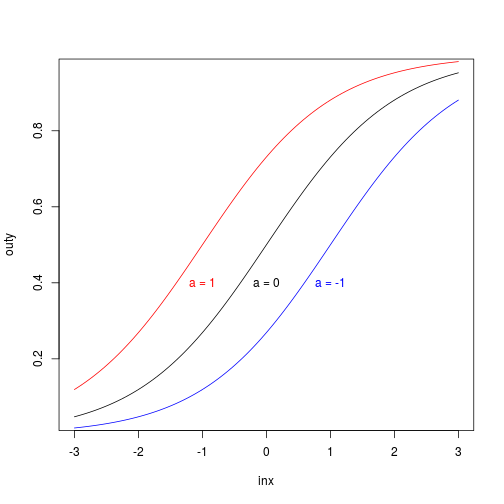
\includegraphics{figure/logitplots1-1.png}
\caption{Different values of \(a\)}
\end{figure}

\subsection{Visually\ldots{}}\label{visually-1}

\(b\) = the degree to which the outcome depends on \(x\)

\begin{figure}[htbp]
\centering
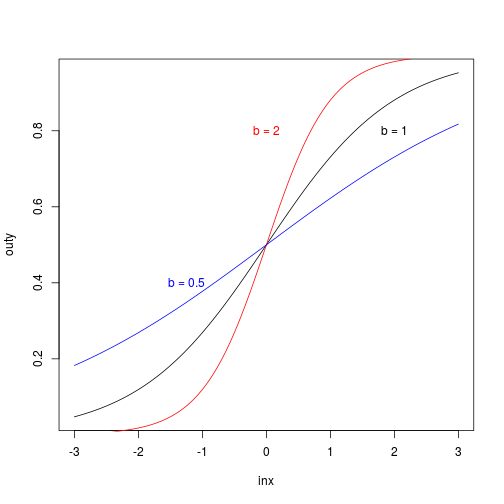
\includegraphics{figure/logitplots2-1.png}
\caption{Different values of \(b\)}
\end{figure}

\subsection{An application}\label{an-application}

\begin{quote}
Gaudet, Frederick, Harris, George S., and St.~John, Charles W. (1933),
``Individual differences in the sentencing tendencies of judges'',
\emph{American Institute of Criminal Law and Criminology}, 23(5),
811-818.
\end{quote}

To my knowledge, the earliest use of random assignment of judges to
investigate judge effects.

\subsection{The logic, explained}\label{the-logic-explained}

\begin{quote}
``Since the rule is that there is no selection of the cases which the
judge is to sentence, but that the sentencing of a particular prisoner
by a particular judge is a matter of chance (the judges rotate), it is
obvious that, by chance, each judge should get an equal number of cases
whose sentences would normally be long or short\ldots{} Given a
sufficiently large number of cases, if one finds that the average
severity of the sentences of two judges is appreciably different, one is
justified in saying that the factors which determine this difference in
the sentencing tendencies are to be found outside of the circumstances
of the crime and those of the prisoner, and hence probably in the judge
since he is the other factor which is always present''.
\end{quote}

\subsection{The table}\label{the-table}

\begin{figure}[htbp]
\centering
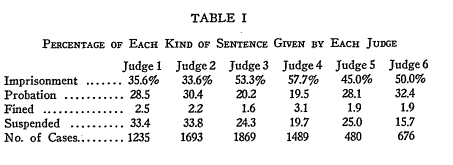
\includegraphics{figure/gaudet_tab1.png}
\caption{Gaudet et al., Fig. 1}
\end{figure}

\subsection{Running a model}\label{running-a-model}

\begin{itemize}
\tightlist
\item
  My focus is on the decision to imprison
\item
  I'll assume this is data from a sample, not the entire population
\item
  Interest is not in the differences, but in their statistical
  significance
\end{itemize}

\subsection{How it looks: the data}\label{how-it-looks-the-data}

\begin{Shaded}
\begin{Highlighting}[]
\NormalTok{gaudet <-}\StringTok{ }\KeywordTok{read.csv}\NormalTok{(}\StringTok{"data/gaudet.csv"}\NormalTok{)}
\KeywordTok{head}\NormalTok{(gaudet)}
\end{Highlighting}
\end{Shaded}

\begin{verbatim}
##     Judge     Sentence
## 1 Judge 1        Other
## 2 Judge 4 Imprisonment
## 3 Judge 2        Other
## 4 Judge 2 Imprisonment
## 5 Judge 1        Other
## 6 Judge 5 Imprisonment
\end{verbatim}

\subsection{How it looks, the model}\label{how-it-looks-the-model}

\begin{Shaded}
\begin{Highlighting}[]
\NormalTok{mod <-}\StringTok{ }\KeywordTok{glm}\NormalTok{(}\KeywordTok{I}\NormalTok{(Sentence ==}\StringTok{ "Imprisonment"}\NormalTok{)~Judge,}
           \DataTypeTok{family =} \NormalTok{binomial,}
           \DataTypeTok{data =} \NormalTok{gaudet)}
\end{Highlighting}
\end{Shaded}

where

\begin{itemize}
\tightlist
\item
  \texttt{glm}: short for \emph{g}eneralized \emph{l}inear \emph{m}odel
\item
  \texttt{I(.)}: what follows isn't just a variable name
\item
  \texttt{family\ =\ binomial}: this is a logistic regression, not some
  other model
\end{itemize}

\subsection{How it looks, the results}\label{how-it-looks-the-results}

\footnotesize

\begin{Shaded}
\begin{Highlighting}[]
\KeywordTok{summary}\NormalTok{(mod)}
\end{Highlighting}
\end{Shaded}

\begin{verbatim}
## 
## Call:
## glm(formula = I(Sentence == "Imprisonment") ~ Judge, family = binomial, 
##     data = gaudet)
## 
## Deviance Residuals: 
##     Min       1Q   Median       3Q      Max  
## -1.3116  -1.0935  -0.9051   1.1220   1.4767  
## 
## Coefficients:
##              Estimate Std. Error z value Pr(>|z|)    
## (Intercept)  -0.59157    0.05942  -9.956  < 2e-16 ***
## JudgeJudge 2 -0.08920    0.07860  -1.135 0.256419    
## JudgeJudge 3  0.72338    0.07537   9.598  < 2e-16 ***
## JudgeJudge 4  0.90162    0.07926  11.376  < 2e-16 ***
## JudgeJudge 5  0.39090    0.10931   3.576 0.000349 ***
## JudgeJudge 6  0.59157    0.09720   6.086 1.16e-09 ***
## ---
## Signif. codes:  0 '***' 0.001 '**' 0.01 '*' 0.05 '.' 0.1 ' ' 1
## 
## (Dispersion parameter for binomial family taken to be 1)
## 
##     Null deviance: 10267.4  on 7441  degrees of freedom
## Residual deviance:  9979.7  on 7436  degrees of freedom
## AIC: 9991.7
## 
## Number of Fisher Scoring iterations: 4
\end{verbatim}

\subsection{How it looks, as published}\label{how-it-looks-as-published}

TODO:

\subsection{Interpretation}\label{interpretation-3}

\begin{itemize}
\tightlist
\item
  The coefficient on Judge 3 is 0.723
\item
  This means that Judge 3 is \(e^{0.723} = 2.061\) times more likely to
  send people to prison.
\item
  That makes sense given the figures listed in Gaudet et al's Table 1.
\end{itemize}

\section{Multiple judges}\label{multiple-judges}

\subsection{Our new source of data}\label{our-new-source-of-data}

\begin{figure}[htbp]
\centering
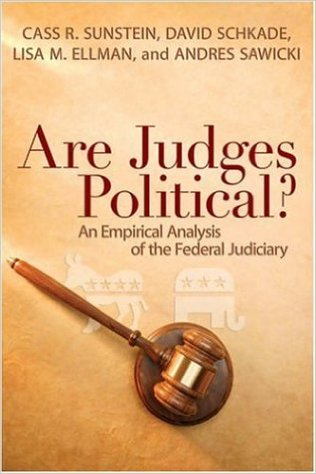
\includegraphics{figure/sunstein_cover.jpg}
\caption{Sunstein et al, \emph{Are judges political?}}
\end{figure}

\subsection{The dependent variable}\label{the-dependent-variable}

\begin{itemize}
\tightlist
\item
  The vote of an individual judge in a case heard by multiple judges
\item
  These votes can be coded in different ways
\item
  Here, the focus is on ``stereotypically liberal'' decisions
\end{itemize}

\subsection{The independent variable}\label{the-independent-variable}

\begin{itemize}
\tightlist
\item
  A dummy variable, which has value one if the judge was appointed by a
  Democratic president
\item
  In the book, this is elided with ideology
\item
  ``Party of the appointing actor'' may be a poor guide in other
  contexts
\end{itemize}

\subsection{The key assumption}\label{the-key-assumption}

\begin{itemize}
\tightlist
\item
  For the book to work, it's necessary for judges to be assigned to
  cases on a random basis
\item
  \emph{Within each circuit}, judges are assigned randomly
\item
  So \emph{within a circuit}, we can just use judge dummies
\end{itemize}

\subsection{A simple example}\label{a-simple-example}

\begin{itemize}
\tightlist
\item
  Let's focus on cases:

  \begin{itemize}
  \tightlist
  \item
    involving the Americans with Disabilities Act
  \item
    in the 7th Circuit
  \end{itemize}
\item
  Why? Most common circuit-casetype combination
\end{itemize}

\begin{Shaded}
\begin{Highlighting}[]
\NormalTok{dat <-}\StringTok{ }\KeywordTok{read.csv}\NormalTok{(}\StringTok{"data/Ch4Sunstein.csv"}\NormalTok{)}
\NormalTok{ada <-}\StringTok{ }\KeywordTok{subset}\NormalTok{(dat, circuit ==}\StringTok{ }\DecValTok{7} \NormalTok{&}\StringTok{ }\NormalTok{dataset ==}\StringTok{ }\DecValTok{2}\NormalTok{)}
\KeywordTok{head}\NormalTok{(ada[,}\KeywordTok{c}\NormalTok{(}\StringTok{"judge_name"}\NormalTok{, }\StringTok{"conserve_vote"}\NormalTok{, }\StringTok{"cite"}\NormalTok{, }\StringTok{"dec_year"}\NormalTok{, }\StringTok{"party_pres"}\NormalTok{)])}
\end{Highlighting}
\end{Shaded}

\subsection{A simple model}\label{a-simple-model}

\footnotesize

\begin{Shaded}
\begin{Highlighting}[]
\NormalTok{mod <-}\StringTok{ }\KeywordTok{glm}\NormalTok{(conserve_vote~party_pres,}
           \DataTypeTok{data =} \NormalTok{ada,}
           \DataTypeTok{family =} \NormalTok{binomial)}
\KeywordTok{summary}\NormalTok{(mod)}
\end{Highlighting}
\end{Shaded}

\begin{verbatim}
## 
## Call:
## glm(formula = conserve_vote ~ party_pres, family = binomial, 
##     data = ada)
## 
## Deviance Residuals: 
##     Min       1Q   Median       3Q      Max  
## -1.7268   0.7143   0.7143   0.7143   0.8530  
## 
## Coefficients:
##             Estimate Std. Error z value Pr(>|z|)    
## (Intercept)   1.2359     0.1295   9.547   <2e-16 ***
## party_pres   -0.4122     0.2241  -1.839   0.0659 .  
## ---
## Signif. codes:  0 '***' 0.001 '**' 0.01 '*' 0.05 '.' 0.1 ' ' 1
## 
## (Dispersion parameter for binomial family taken to be 1)
## 
##     Null deviance: 541.56  on 482  degrees of freedom
## Residual deviance: 538.24  on 481  degrees of freedom
## AIC: 542.24
## 
## Number of Fisher Scoring iterations: 4
\end{verbatim}

\subsection{Multiple circuits}\label{multiple-circuits}

\begin{itemize}
\tightlist
\item
  Here, we have results that are not significant at commonly-accepted
  levels
\item
  We have additional data we can use -- data from other circuits
\item
  However, judges are not randomly-assigned to cases \emph{across
  circuits}
\item
  In particular, the chances of a Democrat sitting on certain cases is
  higher on certain circuits
\end{itemize}

\subsection{\texorpdfstring{Testing random assignment \emph{across}
circuits}{Testing random assignment across circuits}}\label{testing-random-assignment-across-circuits}

\begin{itemize}
\tightlist
\item
  Let's model \texttt{party\_pres} as a function of circuit!
\end{itemize}

\begin{Shaded}
\begin{Highlighting}[]
\NormalTok{mod <-}\StringTok{ }\KeywordTok{glm}\NormalTok{(party_pres ~}\StringTok{ }\KeywordTok{factor}\NormalTok{(circuit),}
           \DataTypeTok{data =} \NormalTok{dat,}
           \DataTypeTok{family =} \NormalTok{binomial)}
\end{Highlighting}
\end{Shaded}

\subsection{\texorpdfstring{The ``reverse''
model}{The reverse model}}\label{the-reverse-model}

\scriptsize

\begin{verbatim}
## 
## Call:
## glm(formula = party_pres ~ factor(circuit), family = binomial, 
##     data = dat)
## 
## Deviance Residuals: 
##     Min       1Q   Median       3Q      Max  
## -1.3790  -0.9420  -0.7846   1.3005   1.6299  
## 
## Coefficients:
##                   Estimate Std. Error z value Pr(>|z|)    
## (Intercept)       -0.63777    0.07174  -8.890  < 2e-16 ***
## factor(circuit)2   0.83478    0.09485   8.801  < 2e-16 ***
## factor(circuit)3   0.05505    0.11059   0.498 0.618655    
## factor(circuit)4   0.26836    0.10649   2.520 0.011738 *  
## factor(circuit)5  -0.14806    0.09470  -1.564 0.117927    
## factor(circuit)6   0.69524    0.09349   7.437 1.03e-13 ***
## factor(circuit)7  -0.38275    0.08530  -4.487 7.21e-06 ***
## factor(circuit)8  -0.21268    0.08601  -2.473 0.013408 *  
## factor(circuit)9   1.10016    0.09250  11.894  < 2e-16 ***
## factor(circuit)10  0.35299    0.09598   3.678 0.000235 ***
## factor(circuit)11  0.15504    0.09811   1.580 0.114061    
## factor(circuit)12  0.23834    0.10573   2.254 0.024175 *  
## ---
## Signif. codes:  0 '***' 0.001 '**' 0.01 '*' 0.05 '.' 0.1 ' ' 1
## 
## (Dispersion parameter for binomial family taken to be 1)
## 
##     Null deviance: 18619  on 13927  degrees of freedom
## Residual deviance: 17897  on 13916  degrees of freedom
## AIC: 17921
## 
## Number of Fisher Scoring iterations: 4
\end{verbatim}

\subsection{How to proceed?}\label{how-to-proceed}

\begin{itemize}
\tightlist
\item
  We have seen the chances of a Democrat sitting on a case varies
  according to circuit
\item
  Differences in the rates at which Democrats vote certain ways may
  therefore be due not to party\ldots{}
\item
  but to the types of circuits which Democrats sit on, and the types of
  cases heard by those circuits
\item
  \ldots{} but if we were prepared to say that the chance of a Democrat
  was random \emph{conditional} on knowing the circuit?
\end{itemize}

\subsection{A fuller model}\label{a-fuller-model}

\begin{Shaded}
\begin{Highlighting}[]
\NormalTok{mod <-}\StringTok{ }\KeywordTok{glm}\NormalTok{(conserve_vote~party_pres+}\KeywordTok{factor}\NormalTok{(circuit),}
           \DataTypeTok{data =} \NormalTok{dat,}
           \DataTypeTok{family =} \NormalTok{binomial)}
\end{Highlighting}
\end{Shaded}

\subsection{The fuller model, results}\label{the-fuller-model-results}

\tiny

\begin{Shaded}
\begin{Highlighting}[]
\KeywordTok{summary}\NormalTok{(mod)}
\end{Highlighting}
\end{Shaded}

\begin{verbatim}
## 
## Call:
## glm(formula = conserve_vote ~ party_pres + factor(circuit), family = binomial, 
##     data = dat)
## 
## Deviance Residuals: 
##     Min       1Q   Median       3Q      Max  
## -1.5312  -1.2387   0.8609   1.0497   1.4793  
## 
## Coefficients:
##                   Estimate Std. Error z value Pr(>|z|)    
## (Intercept)        0.36547    0.07019   5.207 1.92e-07 ***
## party_pres        -0.45017    0.03638 -12.373  < 2e-16 ***
## factor(circuit)2  -0.22262    0.09328  -2.387  0.01700 *  
## factor(circuit)3  -0.53767    0.10748  -5.003 5.66e-07 ***
## factor(circuit)4   0.07786    0.10458   0.744  0.45660    
## factor(circuit)5   0.28194    0.09109   3.095  0.00197 ** 
## factor(circuit)6  -0.05747    0.09187  -0.626  0.53158    
## factor(circuit)7   0.43612    0.08148   5.352 8.68e-08 ***
## factor(circuit)8   0.38977    0.08281   4.707 2.52e-06 ***
## factor(circuit)9  -0.60184    0.09122  -6.598 4.17e-11 ***
## factor(circuit)10 -0.16039    0.09382  -1.709  0.08737 .  
## factor(circuit)11  0.15153    0.09575   1.583  0.11353    
## factor(circuit)12 -0.21445    0.10312  -2.080  0.03755 *  
## ---
## Signif. codes:  0 '***' 0.001 '**' 0.01 '*' 0.05 '.' 0.1 ' ' 1
## 
## (Dispersion parameter for binomial family taken to be 1)
## 
##     Null deviance: 19105  on 13918  degrees of freedom
## Residual deviance: 18471  on 13906  degrees of freedom
##   (9 observations deleted due to missingness)
## AIC: 18497
## 
## Number of Fisher Scoring iterations: 4
\end{verbatim}

\subsection{Problems with the analysis in Sunstein et
al.}\label{problems-with-the-analysis-in-sunstein-et-al.}

\begin{itemize}
\tightlist
\item
  Random allocation isn't true even within circuits!
\item
  For information on this, see:
\end{itemize}

\begin{quote}
Hall, M. (2010). Randomness Reconsidered: Modeling Random Judicial
Assignment in the US Courts of Appeals. \emph{Journal of Empirical Legal
Studies}, 7(3), 574-589.
\end{quote}

\begin{itemize}
\tightlist
\item
  Hall called the clerks in each circuit
\item
  He found that ``{[}r{]}andom assignment was not used in the Fourth
  Circuit before the year 2000,the Fifth and Eighth Circuits before
  2003, or the Tenth Circuit before 1998''
\item
  He also noted that partisan composition \emph{of circuits} changes
  over time
\item
  When corrected for these oversights, the magnitude of the effect
  changes.
\item
  Always check the veracity of any random allocation assumption!
\end{itemize}

\section{Panel outcomes}\label{panel-outcomes}

\subsection{A further problem with
Sunstein}\label{a-further-problem-with-sunstein}

\begin{itemize}
\tightlist
\item
  Often, the idea of random assignment is bound up with the idea of a
  randomized controlled trial
\item
  In this context, experimental \emph{subjects} are assigned to a
  treatment or control \emph{condition}
\item
  Subsequent properties of the subjects are measured.
\item
  In Sunstein et al, cases are assign to a treatment (Democratic judge)
  or control (Republican judge)
\item
  \ldots{} but they receive other treatments (the other two judges on
  the panel)
\item
  and the outcome is measured at the level of the treatment (the judge),
  not the case!
\end{itemize}

\subsection{Explaining panel outcomes}\label{explaining-panel-outcomes}

\begin{itemize}
\tightlist
\item
  Ideally, we'd like a way of explaining the effect of judges on panel
  outcomes
\item
  This is problematic, because it requires a theory of panel
  decision-making
\item
  Suppose the median voter decides, and we assign a third judge to an
  existing panel:

  \begin{itemize}
  \tightlist
  \item
    If the two judges are RR, the median judge is R. Adding another R or
    D makes no difference
  \item
    If the two judges are DD, the median judge is D; the same reasoning
    follows
  \item
    If the two judges are RD or DR, adding another D or R will determine
    the median judge
  \end{itemize}
\item
  Only in the last case does the judge matter
\item
  If we ran a regression, and if all circumstances were equally
  probably, our estimate would be biased downwards
\end{itemize}

\subsection{Options}\label{options}

\begin{itemize}
\tightlist
\item
  Option 1 (low-tech): split the data up according to the partisanship
  of the first two judges:

  \begin{itemize}
  \tightlist
  \item
    Pro: Easy to implement
  \item
    Pro: Recovers coefficients which link to the outcome
  \item
    Con: We're left with three effects
  \item
    Con: It's essential atheoretical
  \end{itemize}
\item
  Option 2 (high-tech): posit a latent ideology associated with each
  judge, and take the median

  \begin{itemize}
  \tightlist
  \item
    Pro: matches theory
  \item
    Pro: recovers a single estimate
  \item
    Con: requires some difficult-to-implement Bayesian statistics
  \end{itemize}
\end{itemize}

\subsection{Modelling panel outcomes}\label{modelling-panel-outcomes}

For more information on this type of approach, see:

Hangartner, Dominik, Benjamin E. Lauderdale, and Judith Spirig.
``Refugee Roulette Revisited: Judicial Preference Variation and
Aggregation on the Swiss Federal Administrative Court 2007-2012.''
(Working paper).

\section{Conclusions}\label{conclusions}

\subsection{General}\label{general}

\begin{itemize}
\tightlist
\item
  We've been able to exploit random assignment to learn something about
  judges
\item
  Given (limited, predictable) non-random assignment, we've been able to
  control for that, and still learn
\item
  We haven't discussed strongly non-random assignment (on the basis of
  experience, or other factors).
\end{itemize}

\subsection{Data}\label{data}

\begin{itemize}
\tightlist
\item
  All the data is available on GitHub
\item
  The url is TODO:
\item
  The R code is also there
\item
  The Sunstein data is in any case available at
  \url{http://epstein.wustl.edu/research/behaviorJudges/chapters.php?req=11}
\end{itemize}

\hypertarget{refs}{}

\end{document}
